\documentclass{article}
\usepackage{graphicx} % Required for inserting fig
\usepackage{subfig}
\usepackage{hyperref}

\setlength{\parskip}{16pt}

\title{Final project assignment:\@ Simulation of a base scenario }

\author{Jef Jacobs \\ Toon Eeraerts \\ Wout Deleu}
\date{Semester 2}

\begin{document}
\setlength{\parindent}{0pt} \maketitle \tableofcontents \newpage %geen indent bij nieuwe paragraaf

\maketitle
\newpage

\section{Introduction}
During this report, the final assignment of the `Yard storage assignment
problem' will be discussed. Over the course of past labs, a serious amount of
work and effort went in to designing a simulation which could visualise a given
port complex. The simulation is focused on the storage situation of this yard.
During this report, the basics design choices will be discussed, as well as the
results of the simulation. The basic technology used is Python. The code is
written as dynamic as possible, using global variables and booleans to variate
parameters and the overall flow of the simulation. It is based on a discrete
event simulation, with the possibility of online simulation. To refresh the
situation in brief, the goal is to simulate a yard, in which
containergroups\footnote{Containers arrive only in group. Containers are
    usually not looked at individually. This means they can’t be split up most of
    the time, they are stored in the same place, they enter and leave the yard at
    the same time.} come and go. They can arrive from vessels or from trucks and
trains. Each container needs to be stored on the yard for a specific duration.
The goal is to simulate the storage in the yard, as a result of the in and out
flow.

To recap, during the first lab, the main focus was on the samples that the
existing data brought along. The intention was to be able to sample them in the
further course of the project, in order to approximate reality. During the
second assignment was the objective to setup a base scenario to simulate, and
get first results. The samples determined in previous sessions were converted
to usable distributions, and where used to generate the parameters that come
with the container arrival and departure schedule. With a basic simulation
scenario, the first results could be examined. Important to note however is
that during the development and design of the sample functions, some minor
errors occurred. The problem originated from a misinterpretation of the graphs
out of the first reports, which led to a big underestimation of the amount of
containers that were generated. This was also insinuated while writing the
second report. However, when designing the final simulation, the mistake came
up again, and normally it was fixed, and it should no longer pose a problem.

The goal of this last assignment is to put all the pieces together, and make
the simulation fully functional and usable. Three extra scenarios are
implemented, which could give some new insights in the way the yard works. And
alongside these extra scenarios and the the solution of the previously made
mistake, a visualisation was implemented. This was one of the core goals of
this last semester and really the cherry on top for this course. It brought the
whole project together, and made all the realisations visible, as well as give
a real insight into the mechanisms of the movements of all the different
elements in this yard.

\section{Probability distributions}
The simulation utilizes probability distributions derived from the input data
provided from a real yard, from Ir. E. Thanos. Each distribution is designed to
have the same average results as the input data. The simulation consists of
generating container group samples, each possessing different characteristics
that are determined by the distributions.

\subsection{Inter arrival time}
The sampling frequency of container groups is a critical parameter in the
simulation. In the original input data, container groups frequently arrived at
the same time on the same vessel, leading to a high occurrence of zero
inter-arrival times, shown in Figure~\ref{fig:inter-arrival times real}.
Consequently, the average inter-arrival time has a very low value of 0.092
hours or 5 minutes and 30 seconds.

To ensure a representative distribution, this average value had to be present
in our sample distribution. To represent the steepness of the graph, an
exponential function was used, resulting in the distribution shown in
Figure~\ref{fig:inter-arrival times sample}.

\begin{figure}[!tbp]
    \centering
    \subfloat[Real distribution]{
        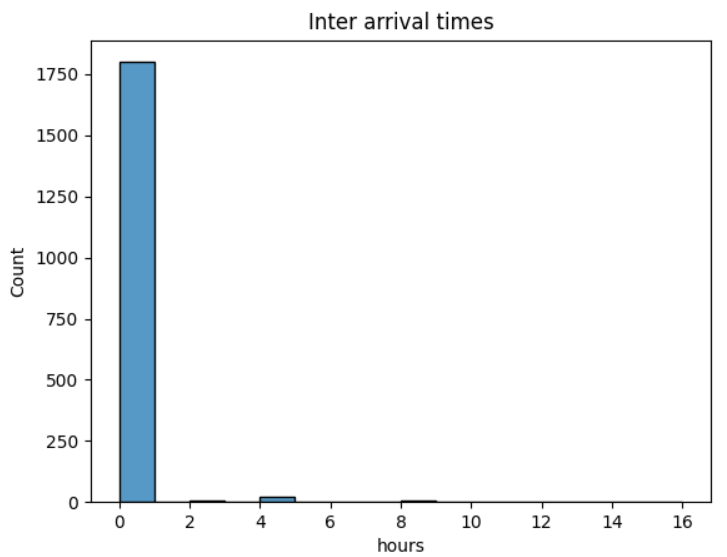
\includegraphics[width=0.48\textwidth]{fig/input data - inter-arrival times.png}\label{fig:inter-arrival times real}}
    \hfill
    \subfloat[Sample distribution]{
        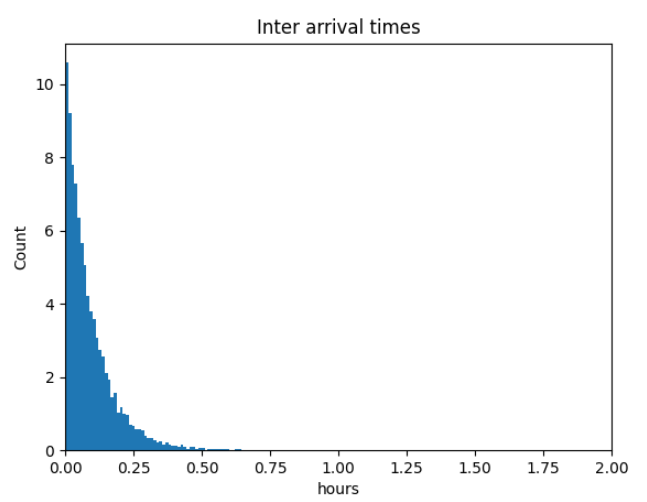
\includegraphics[width=0.48\textwidth]{fig/sample inter-arrival times.png}\label{fig:inter-arrival times sample}}
    \caption{Inter-arrival times}
\end{figure}

\subsection{Container group size}
The container group sizes in the input data indicate significant variance,
ranging from single-container groups to groups with over 2000 containers. This
strong variance caused a difficult decision in determining an appropriate
distribution. In the end, a Weibull distribution was chosen to achieve a steep
descent at the lower end while simultaneously allowing for the possibility of
larger group sizes. The average size of container groups in the input data, as
shown in Figure~\ref{fig:cg_sizes_real}, is 32 containers. The Weibull
distribution used for this sample generation is shown in
Figure~\ref{fig:cg_sizes_sample}.

Considering the previous average outcome, we can determine how many containers
are generated each week. This number corresponds to the amount of containers
getting transported each week. The result is almost equal to the amount of
containers from the input data, thereby validating the average values of the
previous distributions.

\begin{equation}
    Generated\_containers = \frac{Total\_time}{inter\_arrival\_time} \cdot Average\_container\_group\_size \end{equation}
\begin{equation} = \frac{168}{0.091} \cdot 32 \end{equation}
\begin{equation} \approx 59000 \end{equation}

\begin{figure}[!tbp]
    \centering
    \subfloat[Real distribution]{
        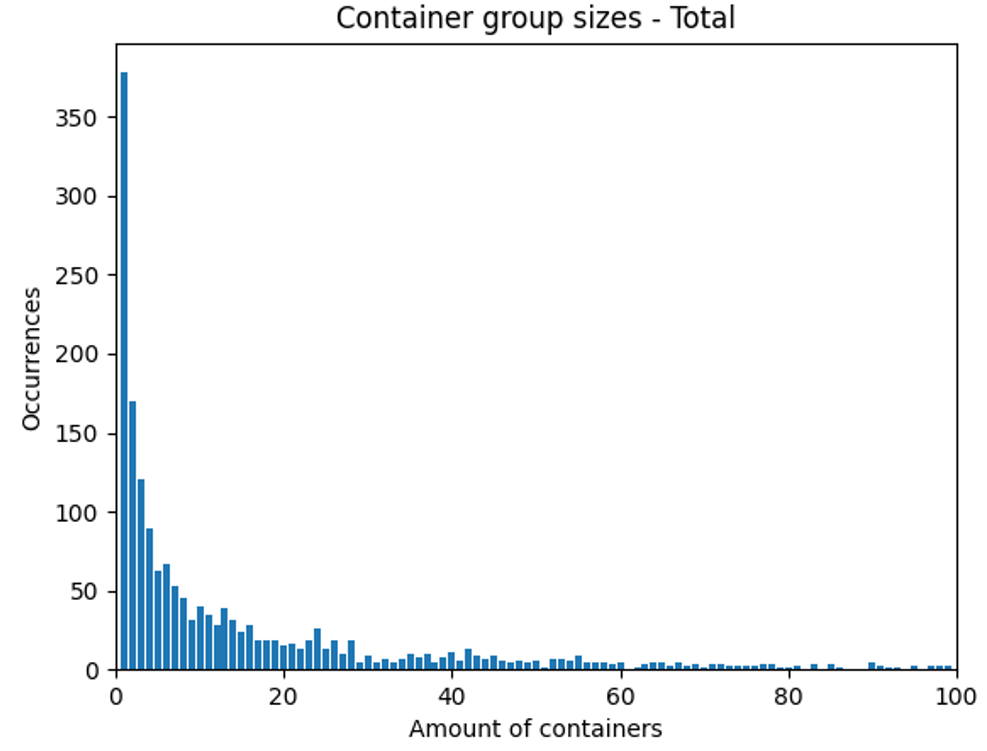
\includegraphics[width=0.48\textwidth]{fig/input data - cg sizes.png}
        \label{fig:cg_sizes_real}}
    \hfill
    \subfloat[Sample distribution]{
        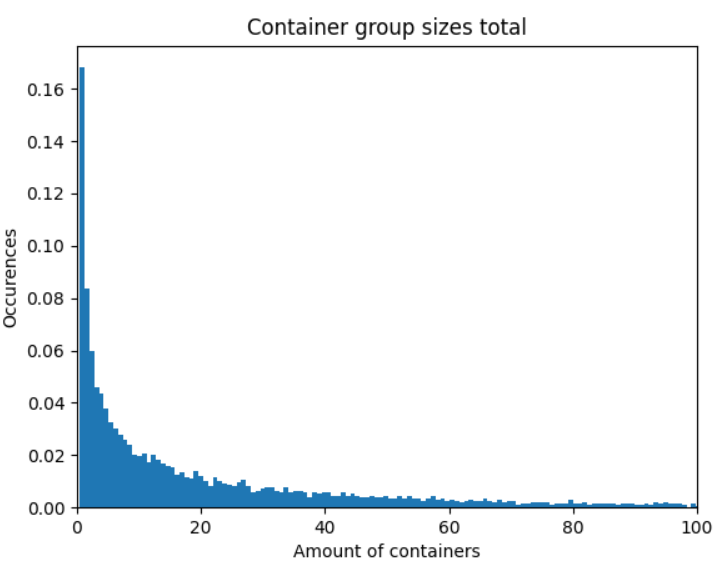
\includegraphics[width=0.48\textwidth]{fig/sample cg sizes.png}
        \label{fig:cg_sizes_sample}}
    \caption{Container group sizes}
\end{figure}

\subsection{Service time}
The service time of each container group represents how long they stay in the
yard before departing. The input data revealed a uniform distribution ranging
from zero to 166 hours, shown in Figure~\ref{fig: service sample distribution}.
However, it is important to note that this distribution solely represents the
container groups falling under transshipment. The other kind of container
groups (export and import) always have a service time of 48 hours.

While it would be interesting to consider generating consistent container
groups with a service time of 48 hours, we chose to simplify the distribution
due to the larger number of transshipment container groups compared to the
other types. The resulting distribution is a unfiorm distribution between zero
and 166 hours.

\begin{figure}
    \centering
    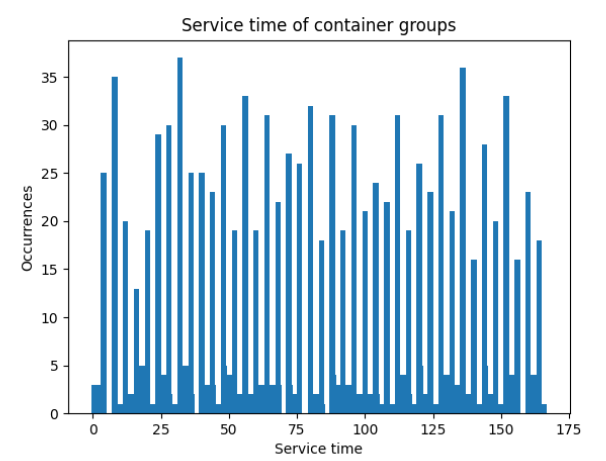
\includegraphics[width=0.5\textwidth]{fig/service time analysis.png}
    \caption{Service time sample distribution}\label{fig: service sample distribution}
\end{figure}

\subsection{Container type}
Each container group can be of normal or reefer type. This distribution was
based upon the input analysis of Nick De Bruyckere, Enrique Miron and Dries Van
de Velde represented in Figure~\ref{fig:container type analysis}. Normal
containers and reefer container occur respectively 69\% and 31\% of the times.

\begin{figure}
    \centering
    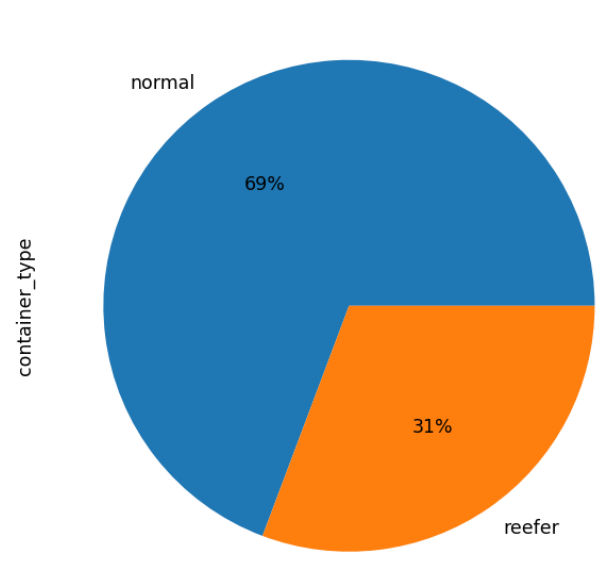
\includegraphics[width=0.5\textwidth]{fig/container_type.png}
    \caption{Container type analysis}\label{fig:container type analysis}
\end{figure}

\subsection{Arrival and departure points}
The arrival and departure positions of vessels and trucks are chosen randomly
from the available locations. The selection of either a vessel location or a
truck location depends on the flow type, which will be discussed later.

\subsection{Flow type}
Each container group can be categorized as either export or import. In the
input data, all groups that were categorized as transshipment are now
categorized as export. The distribution of these flow types is based on the
proportion of containers in the input data belonging to each category,
resulting in 81\% export and 19\% import.

For the container groups classified as export, further division was necessary
to determine their berthing locations and potential truck locations. This is
because transshipment's would go from vessel to vessel, while true exports from
truck to vessel. This distribution resulted in 69\% transshipment's and 31\%
true export.

\section{Algorithm}
In this section the flow and the architectural and design will be elaborated
and discussed. Because this code was designed over different steps, with it's
own goals, the program tends to be very modular. This is particularly handy for
possible code reuse for now or in the future.
\subsection{Amount of simulations}
The first and maybe most primary parameter to know is the amount of simulations
that needs to be run to get significant results. This can be calculated by the
following formula: \[S = \sqrt{\frac{\sum_{i = 1}^{n}(X_i-\overline{X})^2}{n
            -1}}\] \[\frac{S}{\sqrt{k}} < d\]

The resulting value of the simulation we wanted to take in account, is the
travel distance. S the sample variance, the variance of our results. The number
of simulations, so the value we want to calculate is k. The accepted standard
deviation is d. This is a threshold we want to achieve, and can be chosen in
function of the given results. X represents a system result of the simulation.
In our case is this the average or total travel distance gotten from running
the simulation. When the sample variance based on the k values is within an
acceptable range, the calculation is stopped and the value of k is chosen for
the amount of simulations that needs to be run.

For the total distance the accepted deviation is 1000. If we look at the
magnitude of the total travel distance, we see it surpasses a million. A
deviation of a thousands seems in that case reasonable. The total distance
travelled is a much larger value than the average, because of this the accepted
deviation is larger. From this information we can conclude that at least 120
simulations must be done to get consistent results.

\begin{figure}[h]
    \centering
    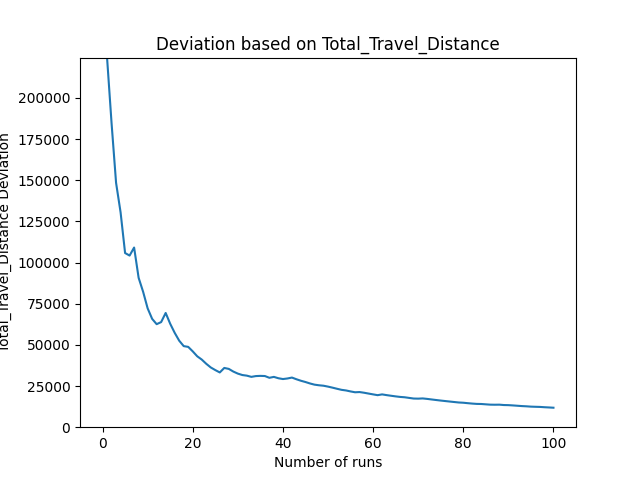
\includegraphics[width=0.7\textwidth]{fig/calcruns.png}
    \caption{Deviation based on total travel distance}\label{fig:amount_of_runs}
\end{figure}

\subsection{Flow}
Because of the nature of a simulation, where multiple scenarios need to be
tested, it was a challenge to design and structure the program in such a way
that the flow could be manipulated without making drastic internal changes. The
flow can be manipulated by the use of booleans which map out the path. Checks
are present to throw Exceptions, so that the booleans (which are some sort of
input parameters, and are in the GUI implemented in this way, but more on that
later) can only be configured in such a way that they map out a predefined
scenario. Here 4 booleans where used:
\begin{enumerate}
    \item ARRIVAL BASED
    \item DEPARTURE BASED
    \item CLOSEST
    \item LOWEST OCCUPANCY
    \item MIXED RULE
    \item SPLIT UP
\end{enumerate}

\subsection{Core}
The program is event based, which means the simulation timer jumps from event
to event. It achieves this by keeping two different list which hold events, one
where containers arrive at the yard, and one where containers depart from the
yard. Every time a container is generated, a new arrival is being scheduled
based on the interarrival time sampling function. When it arrives, it is
checked if it can be placed on a place in the yard. If it can, a yardblock
where it can be stored is selected based on the scenario. If it can't, it is
rejected. At an event where a container departs, the container is removed from
the yard. For every event happening, all the statistics are updated. This
process repeats itself until the simulation time is reached.

\subsection{Visualisation}
The visualisation is done by the use of TKinter. Tkinter is a Python library
used for creating graphical user interfaces (GUIs). The name`Tkinter' comes
from `Tk interface', referring to the fact that it is based on the Tk GUI
toolkit. One of the advantages of Tkinter is that it is included with the
standard Python distribution, so you don't need to install any additional
libraries. This makes it easily accessible for beginners and convenient for
developing cross-platform applications.

Overall, Tkinter is a powerful tool for developing graphical applications in
Python, enabling you to create intuitive and interactive user interfaces for
your programs.

Some keyfeatures of the simulation is that the possibility to setup a flow
using the intro screen, seen in Figure~\ref{fig:intro}. Here you can setup all
the necessary parameters to run a simulation, as well as the duration.
\begin{figure}
    \centering
    \includegraphics[width=0.7\textwidth]{fig/intro_screen.png}
    \caption{Intro screen}\label{fig:intro}
\end{figure}

The visualisation is multithreaded, which allows it to run smooth. It is
possible to run both the visualisation and gatter results formatted in a LaTex
table (which has to be run multiple times to get correct results). But a strong
computer is needed to pull this off. Because of the multithreaded visualisation
was it not usable, but in case of stronger pc's, it should work fluently. More
on performance later in Section~\ref{sec:performance}.
\begin{figure}
    \centering
    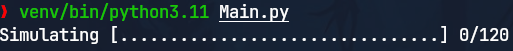
\includegraphics[width=0.7\textwidth]{fig/progressbar.png}
    \caption{Progress bar of the simulations being run in order to get results}\label{fig:visualisation}
\end{figure}

When the graphical representation is running, the boats are represented on the
water on top. They appear and disapear if they are needed. The yard is
represented by the blocks of different size based on their respective capacity,
mostly in flashy green. It is noticable that the reefer blocks are very small.

\section{What-if scenarios}
A significant part of the assignment was to implement some scenarios in order
to look for the most `efficient' scenarios, or more generally speaking, see the
impact of these scenarios. This is also an opportunity to test out the
visualisation, and see in what manner the yard works.

As stated in the previous reports, two different approaches to block
assignments are implemented. This still applies to all the scenarios described
in this section, and so for most scenarios the two different approaches of
block assignment are possible. The block assignment rule has affect on which
block is chosen to store a containergroup. The two different situations studied
here are arrival based and departure based. Arrival based and departure based
are both based on the minimal distance between 2 points. The yard block chosen
is the closest block to the arrival point, in case of arrival based, or closest
to the departure point, in case of departure based.

\subsection{Base Scenario}
The base scenario stays the same as discussed in the previous report, where the
decision rule is that containergroup that arrives, if there is space in the
yard. This will be referred to as FIFO (First In First Out). This apply’s to
arrival of containers, and wether or not they are stored in the yard. FIFO says
that the first container that arrives, has a priority over the ones which
arrive after the first one. If there is no space for an arriving
containergroup, it will be rejected. The block assignment determines which
yardblock the respective containers .

BESCHRIJVEN RESULTATEN...
\begin{table}[h]
    \centering
    \begin{tabular}{|c|c|}
        \hline
        Containers Rejected                         & 548306.083     \\ \hline
        CG Rejected                                 & 4034.933       \\ \hline
        Normal Rejected                             & 9816.133       \\ \hline
        Reefer Rejected                             & 538489.95      \\ \hline
        Total Travel Distance                       & 5314784151.897 \\ \hline
        AVG Travel Distance Containers              & 1754.928       \\ \hline
        Portion of YB close to full (at some point) & 0.698          \\ \hline
        Portion of YB never used                    & 0.195          \\ \hline
        Portion of YB close to full (average)       & 0.698          \\ \hline
        AVG daily total Occupancy                   & 0.745          \\ \hline
    \end{tabular}
    \caption{FIFO ARRIVAL-BASED}
\end{table}
\begin{table}[h]
    \centering
    \begin{tabular}{|c|c|}
        \hline
        Containers Rejected                         & 549260.158    \\ \hline
        CG Rejected                                 & 4029.158      \\ \hline
        Normal Rejected                             & 9932.708      \\ \hline
        Reefer Rejected                             & 539327.45     \\ \hline
        Total Travel Distance                       & 5823736051.32 \\ \hline
        AVG Travel Distance Containers              & 1923.124      \\ \hline
        Portion of YB close to full (at some point) & 0.591         \\ \hline
        Portion of YB never used                    & 0.258         \\ \hline
        Portion of YB close to full (average)       & 0.591         \\ \hline
        AVG daily total Occupancy                   & 0.673         \\ \hline
    \end{tabular}
    \caption{FIFO ARRIVAL-BASEDDEPARTURE-BASED}
\end{table}
\begin{table}[h]
    \centering
    \begin{tabular}{|c|c|}
        \hline
        Containers Rejected                         & 551553.892     \\ \hline
        CG Rejected                                 & 4053.15        \\ \hline
        Normal Rejected                             & 12869.05       \\ \hline
        Reefer Rejected                             & 538684.842     \\ \hline
        Total Travel Distance                       & 6622102730.796 \\ \hline
        AVG Travel Distance Containers              & 2184.101       \\ \hline
        Portion of YB close to full (at some point) & 0.648          \\ \hline
        Portion of YB never used                    & 0.05           \\ \hline
        Portion of YB close to full (average)       & 0.648          \\ \hline
        AVG daily total Occupancy                   & 0.842          \\ \hline
    \end{tabular}
    \caption{FIFO DEPARTURE-BASED}
\end{table}

\subsection{Smallest Remaining capacity}
The first new scenario is one where all containers of the same containergroup
must be stored in the same yardblock. The containers are stored in the
yardblock with the largest remaining capacity, which means the yard should fill
up gradually and balanced over all the possible storage blocks. Due to the lack
of explicit emphasis, two possible interpretations were available for the
"remaining capacity" concept. In this implementation, the choice was made to
work with the absolute number of available container slots. An alternative
interpretation could have been to consider normalized remaining capacity, in
other words, the percentage of capacity that is still available. In case there
are two yardblocks with the exact same capacity left, the closest one is taken
(based on the block assignment rule).

BESCHRIJVEN RESULTATEN...
\begin{table}[h]
    \centering
    \begin{tabular}{|c|c|}
        \hline
        Containers Rejected                         & 650443.533     \\ \hline
        CG Rejected                                 & 5013.842       \\ \hline
        Normal Rejected                             & 48756.217      \\ \hline
        Reefer Rejected                             & 601687.317     \\ \hline
        Total Travel Distance                       & 8270153316.425 \\ \hline
        AVG Travel Distance Containers              & 2728.917       \\ \hline
        Portion of YB close to full (at some point) & 0.453          \\ \hline
        Portion of YB never used                    & 0.245          \\ \hline
        Portion of YB close to full (average)       & 0.453          \\ \hline
        AVG daily total Occupancy                   & 0.645          \\ \hline
    \end{tabular}
    \caption{LOWEST OCCUPANCY ARRIVAL \& DEPARTURE-BASED}
\end{table}

\begin{table}[h]
    \centering
    \begin{tabular}{|c|c|}
        \hline
        Containers Rejected                         & 651509.433     \\ \hline
        CG Rejected                                 & 5014.367       \\ \hline
        Normal Rejected                             & 49211.8        \\ \hline
        Reefer Rejected                             & 602297.633     \\ \hline
        Total Travel Distance                       & 8268808654.143 \\ \hline
        AVG Travel Distance Containers              & 2725.312       \\ \hline
        Portion of YB close to full (at some point) & 0.447          \\ \hline
        Portion of YB never used                    & 0.245          \\ \hline
        Portion of YB close to full (average)       & 0.447          \\ \hline
        AVG daily total Occupancy                   & 0.646          \\ \hline
    \end{tabular}
    \caption{LOWEST OCCUPANCY DEPARTURE-BASED}
\end{table}

\begin{table}[h]
    \centering
    \begin{tabular}{|c|c|}
        \hline
        Containers Rejected                         & 650775.533     \\ \hline
        CG Rejected                                 & 5008.1         \\ \hline
        Normal Rejected                             & 48856.217      \\ \hline
        Reefer Rejected                             & 601919.317     \\ \hline
        Total Travel Distance                       & 8263128846.329 \\ \hline
        AVG Travel Distance Containers              & 2725.798       \\ \hline
        Portion of YB close to full (at some point) & 0.465          \\ \hline
        Portion of YB never used                    & 0.245          \\ \hline
        Portion of YB close to full (average)       & 0.465          \\ \hline
        AVG daily total Occupancy                   & 0.647          \\ \hline
    \end{tabular}
    \caption{LOWEST OCCUPANCY ARRIVAL-BASED}
\end{table}

\subsection{Possible split ups}
This scenario states that containergroups could possibly be split up into
individual containers, which each of which can be considered separately. This
means that a yardblock does not has to hold a full group, so this means larger
containergroups should be handled far more easy. Also the smaller yardblock
should be able to have more use in the grand scheme of things. The yardblocks
chosen to store containers, are the blocks closest to the arrival or departure
point (based on the decision rule), and which have space left to store one or
more containers. So the focus is really on which block is the closest, and can
hold one or more containers.

BESCHRIJVEN RESULTATEN...

\subsection{Not allowing mixing container types in a single yardblock}
The last discussed scenario involves a rule where MIX yardblocks can only serve
containers of a single flow type. This means that ones a container arrives and
takes place in a mix type yardblock, only containers with the same type can be
added to this yardblock.

BESCHRIJVEN RESULTATEN...

\begin{table}[h]
    \centering
    \begin{tabular}{|c|c|}
        \hline
        Containers Rejected                         & 562005.908     \\ \hline
        CG Rejected                                 & 4285.208       \\ \hline
        Normal Rejected                             & 10305.508      \\ \hline
        Reefer Rejected                             & 551700.4       \\ \hline
        Total Travel Distance                       & 5329012083.215 \\ \hline
        AVG Travel Distance Containers              & 1757.727       \\ \hline
        Portion of YB close to full (at some point) & 0.679          \\ \hline
        Portion of YB never used                    & 0.176          \\ \hline
        Portion of YB close to full (average)       & 0.679          \\ \hline
        AVG daily total Occupancy                   & 0.748          \\ \hline
    \end{tabular}
    \caption{MIXED RULE ARRIVAL-BASED}
\end{table}

\begin{table}[h]
    \centering
    \begin{tabular}{|c|c|}
        \hline
        Containers Rejected                         & 562459.5       \\ \hline
        CG Rejected                                 & 4311.817       \\ \hline
        Normal Rejected                             & 12785.225      \\ \hline
        Reefer Rejected                             & 549674.275     \\ \hline
        Total Travel Distance                       & 6606445719.566 \\ \hline
        AVG Travel Distance Containers              & 2180.617       \\ \hline
        Portion of YB close to full (at some point) & 0.648          \\ \hline
        Portion of YB never used                    & 0.044          \\ \hline
        Portion of YB close to full (average)       & 0.648          \\ \hline
        AVG daily total Occupancy                   & 0.842          \\ \hline
    \end{tabular}
    \caption{MIXED RULE DEPARTURE-BASED}
\end{table}

\begin{table}[h]
    \centering
    \begin{tabular}{|c|c|}
        \hline
        Containers Rejected                         & 557756.75     \\ \hline
        CG Rejected                                 & 4226.058      \\ \hline
        Normal Rejected                             & 9384.333      \\ \hline
        Reefer Rejected                             & 548372.417    \\ \hline
        Total Travel Distance                       & 5823224027.74 \\ \hline
        AVG Travel Distance Containers              & 1922.426      \\ \hline
        Portion of YB close to full (at some point) & 0.61          \\ \hline
        Portion of YB never used                    & 0.245         \\ \hline
        Portion of YB close to full (average)       & 0.61          \\ \hline
        AVG daily total Occupancy                   & 0.678         \\ \hline
    \end{tabular}
    \caption{MIXED RULE ARRIVAL-BASED DEPARTURE-BASED}
\end{table}

\section{Performance}\label{sec:performance}

zeggen python suckt Average time per simulation: 127.2401417116324 seconds

\end{document}